%%%%%%%%%%%%%%%%%%%%%%%%%%%%%%%%%%%%%%%%%%%%%%%%%%%%%%%%%%%%%%%%%%%%%%%%%%%%%%%
% Chapter 3: Procedimiento experimental 
%%%%%%%%%%%%%%%%%%%%%%%%%%%%%%%%%%%%%%%%%%%%%%%%%%%%%%%%%%%%%%%%%%%%%%%%%%%%%%%

Este cap�tulo ha de contar con seccciones para la descripci�n de los experimentos 
y del material.
%
Tambi�n debe haber una secci�n para los resultados obtenidos y una �ltima de 
an�lisis de los resultados.

%++++++++++++++++++++++++++++++++++++++++++++++++++++++++++++++++++++++++++++++
\section{Descripci�n de los experimentos}
\label{3:sec:1}

bla, bla, etc. 

%++++++++++++++++++++++++++++++++++++++++++++++++++++++++++++++++++++++++++++++
\section{Descripci�n del material}
\label{3:sec:2}

bla, bla, etc. 


%++++++++++++++++++++++++++++++++++++++++++++++++++++++++++++++++++++++++++++++
\section{Resultados obtenidos}
\label{3:sec:3}

bla, bla, etc. 


%------------------------------------------------------------------------------
\begin{figure}[!th]
\begin{center}
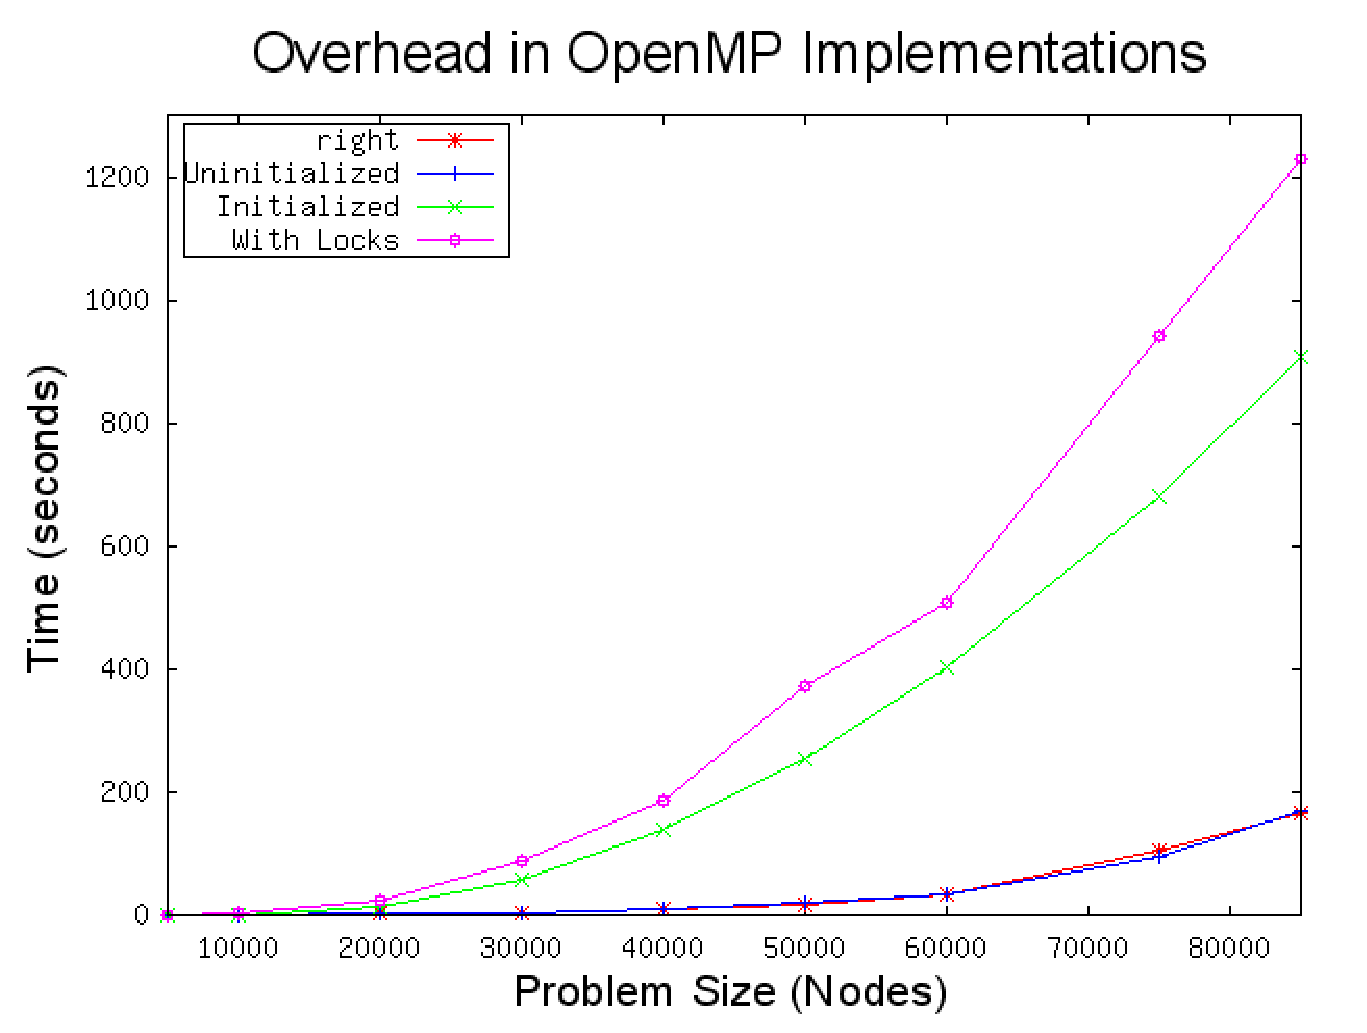
\includegraphics[width=0.75\textwidth]{images/figura1.eps}
\caption{Ejemplo de figura}
\label{fig:1}
\end{center}
\end{figure}
%------------------------------------------------------------------------------


%------------------------------------------------------------------------------
%--------------------------------------------------------------------------
\begin{table}[!ht]
\begin{center}
\begin{tabular}{|l|c|c|c|c|} \hline 

%Nº dipéptidos & Función observada & Código "Triángulo" & Código "Diamante" & Distribución de Poisson \\ 
N & F & CT & CD & D. Poisson\\ \hline
0 & 264 & 276 & 305 & 264.2 \\ \hline
1 & 103 & 86 & 55 & 116.0 \\ \hline
2 & 27 & 26 & 23 & 25.6 \\ \hline
3 & 4 & 9 & 7 & 3.77 \\ \hline
4 & 2 & 3 & 3 & 0.42 \\ \hline
5 & 0 & 0 & 3 & 0.037 \\ \hline
6 & 0 & 0 & 2 & 0.0027 \\ \hline
7 & 0 & 0 & 0 & $1.7x10^{-4}$\\ \hline
8 & 0 & 0 & 2 & $9.5x10^{-6}$ \\ \hline

\end{tabular}
\end{center}
\caption{Datos}
\label{tabla1}
\end{table}


%------------------------------------------------------------------------------

%++++++++++++++++++++++++++++++++++++++++++++++++++++++++++++++++++++++++++++++
\section{An�lisis de los resultados}
\label{3:sec:4}

bla, bla, etc. 

